\documentclass[a4paper,11pt,fleqn]{article}%fleqn pour aligner les equations à gauche
\usepackage{../../Styles/Cours}

\newcommand{\chnum}{Chapitre 11}
\newcommand{\chtitle}{Décrire un mouvement}
\newcommand{\dtype}{Cours}

\begin{document}
\maketitle

\section{Position, vitesse et accélération}
	\subsection{Référentiel}
\begin{multicols}{2}
Le mouvement d'un objet s'étudie dans un \textbf{référentiel} donné, c'est-à-dire par rapport à un objet servant de référence. À chaque référentiel est associé :
\begin{itemize*}
	\item un \textbf{repère spatial} (point d'origine $O$ et repère orthonormé) qui permet de repérer la position de l'objet
	\item un \textbf{repère temporel} qui permet d'associer une date à chaque position.
\end{itemize*}
Exemples : repères d'espace associés au référentiel terrestre situé à la surface de la Terre (1) et au référentiel géocentrique placé au centre de la Terre (2).

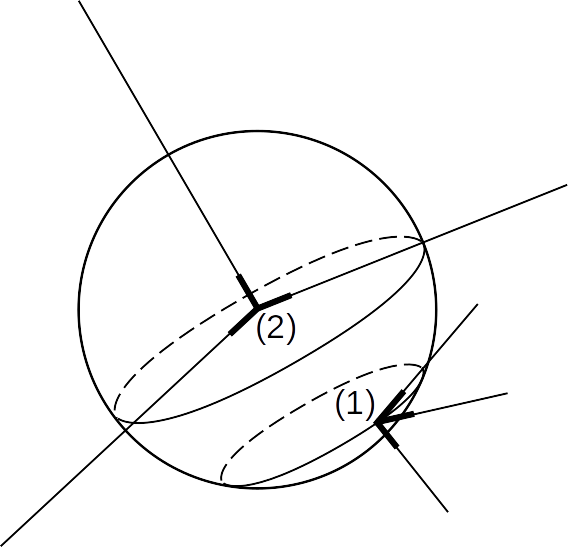
\includegraphics[scale=.3]{Ressources/TSPE_C4_Fig1.png}
\end{multicols}

	\subsection{Position}
Pour faciliter l'étude du mouvement d'un système, celui-ci est modélisé par un point noté \textbf{M}, dont on repérera les coordonnées.\\
\begin{multicols}{2}
	Dans l'espace, le point \textbf{M} se repère à l'aide du \textbf{vecteur position} $\vv{OM}(t)$ dont les coordonnées dans le repère cartésien ($O$, $\vec{i}$, $\vec{j}$, $\vec{k}$) sont :
\begin{multicols}{2}
	$$ \vv{OM}(t) \left\{ \begin{array}{l} x(t) \\ y(t) \\ z(t) \\ \end{array} \right\} _{(O, \vec{i}, \vec{j}, \vec{k})} $$ \\
	$x(t)$ : abscisse du point M\\
	$y(t)$ : ordonnée du point M \\
	$z(t)$ : altitude du point M 
\end{multicols}
L'ensemble des positions occupées par le point $M$ au cours du temps constitue sa \textbf{trajectoire}.

	\begin{tikzpicture}[scale=.5, transform shape]
	\draw (0,0) -- (10,0);
	\draw (0,0) -- (0,10);
	\draw (0,0) -- (-5,-5);
	
	\draw[line width=2pt,green!60!black, -stealth] (0,0) to (0,2);
	\draw[line width=2pt,green!60!black, -stealth] (0,0) to (2,0);
	\draw[line width=2pt,green!60!black, -stealth] (0,0) to (-1.41,-1.41);
	
	\draw[line width=2pt,blue!60!black, -stealth] (0,0) to (5,6); 
	
	\draw[dashed] (5,6) -- (5,-3);
	\draw[dashed] (0,0) -- (5,-3);
	\draw[dashed] (5,6) -- (5,-3);
	\draw[dashed] (0,9) -- (5,6);
	\draw[dashed] (0,0) -- (5,-3);
	\draw[dashed] (-3,-3) -- (5,-3);
	\draw[dashed] (8,0) -- (5,-3);
	
	\node[left] (O) at (-0.2,0){\huge $O$};
	\node[above right] (M) at (5,6){\huge $M(t)$};
	\node[above right,green!60!black](i) at (-.2,-1.2){\huge $\vec{i}$};
	\node[above,green!60!black](j) at (1.2,0) {\huge $\vec{j}$};
	\node[left,green!60!black](k) at (-.2,1){\huge $\vec{k}$};
	\draw (-3,-2.8) -- (-3,-3.2); \node[left] (x) at (-3,-3){\huge $x(t)$};
	\draw (8,-0.2) -- (8,0.2); \node[above] (x) at (8,0){\huge $y(t)$};
	\draw (-0.2,9) -- (0.2,9); \node[left] (x) at (0,9){\huge $z(t)$};
	\end{tikzpicture}
\end{multicols}

	\subsection{Vitesse}
En seconde et en première, le vecteur est définit approximativement comme la variation de la position en fonction du temps :
$$\vec{v} = \dfrac{\vv{MM'}}{\Delta t} = \dfrac{\vv{MO} + \vv{OM'}}{\Delta t} = \dfrac{\vv{OM'} - \vv{OM}}{\Delta t} = \dfrac{\Delta \vv{OM}}{\Delta t} $$

En considérant une durée $\Delta t$ infiniment faible, on aboutit à la notion de dérivée. Ainsi, le \textbf{vecteur vitesse} est définit comme la dérivée temporelle du vecteur position :
$$\vec{v} = \dfrac{d\vv{OM}}{dt}$$
Dans le repère cartésien ($O$, $\vec{i}$, $\vec{j}$, $\vec{k}$), les coordonnées du vecteur vitesse $\vec{v}$ sont :
$$\vec{v}(t)
	\left( 
	\begin{array}{l} v_x(t)=\dfrac{dx}{dt} \\ v_y(t)=\dfrac{dy}{dt} \\ v_z(t)=\dfrac{dz}{dt} \\ 
	\end{array} 
	\right) _{(O, \vec{i}, \vec{j}, \vec{k})}$$
La notation : $\dfrac{dx}{dt}$, $\dfrac{dy}{dt}$, $\dfrac{dz}{dt}$ peut parfois se noter $\dot{x}$, $\dot{y}$, $\dot{z}$.\\

La \textbf{valeur de la vitesse} à une date donnée est également égale à la norme du vecteur $\vec{v}$ :
$$v=\sqrt{v_x^2 + v_y^2 + v_z^2}$$
$$\text{avec } v \text{ en \unit{\meter\per\second}}$$ 

	\subsection{Accélération}
Le \textbf{vecteur accélération} caractérise la variation du vecteur vitesse en fonction du temps. Il est défini comme la dérivée temporelle du vecteur et, par conséquent, comme la dérivée seconde du vecteur position :
$$ \vec{a} = \dfrac{d\vec{v}}{dt} = \dfrac{d^2\vv{OM}}{dt^2}$$
Dans le repère cartésien ($O$, $\vec{i}$, $\vec{j}$, $\vec{k}$), les coordonnées du vecteur accélération $\vec{a}$ sont :
$$\vec{a}(t)
	\left(
	\begin{array}{l}
	a_x(t) = \dfrac{dv_x}{dt} \\ a_y(t) = \dfrac{dv_y}{dt} \\ a_z(t) = \dfrac{dv_z}{dt}\\
	\end{array}
	\right)_{(O, \vec{i}, \vec{j}, \vec{k})}$$

La notation $\dfrac{d^2x}{dt^2}$, $\dfrac{d^2y}{dt^2}$, $\dfrac{d^2z}{dt^2}$ peut parfois se noter $\ddot{x}$, $\ddot{y}$, $\ddot{z}$.\\

La \textbf{valeur de l'accélération} à une date donnée est également égale à la norme du vecteur $\vec{a}$ :
$$a=\sqrt{a_x^2 + a_y^2 + a_z^2}$$
\begin{center} avec $a$ en \unit{\meter\per\second\squared} \end{center}

\section{Étude de quelques cas courants}
	\subsection{Mouvements rectilignes}
		\subsubsection*{Mouvement rectiligne :}
		Un mouvement est rectiligne si sa trajectoire est une droite. Il peut donc être décrit selon un seul axe. Par conséquent, les vecteurs position, vitesse et accélération ne conservent qu'une composante.\\ \emph{Exemple pour un mouvement horizontal :}
		
		$$\vv{OM}(t) = x(t) \cdot \vec{i}$$
		$$\vec{v}(t) = v_x(t) \cdot \vec{i} = \dfrac{dx}{dt} \cdot \vec{i}$$
		$$\vec{a}(t) = a_x(t) \cdot \vec{i} = \dfrac{dv_x}{dt} \cdot \vec{i} =\dfrac{d^2x}{dt^2} \cdot \vec{i}$$
\newpage
		Le vecteur accélération a donc pour caractéristiques :
		\begin{itemize*}
			\item \textit{direction} : droite correspondant à la trajectoire
			\item \textit{sens} : sens du mouvement
			\item \textit{valeur} : $a=\dfrac{dv_x}{dt} = \dfrac{d^2x}{dt^2}$ pour un mouvement horizontal ; $a=\dfrac{dv_z}{dt} = \dfrac{d^2_z}{dt^2}$ pour un mouvement vertical
		\end{itemize*}
		
	\subsubsection*{Mouvement rectiligne uniforme :}

\begin{multicols}{2}
		Un mouvement rectiligne est uniforme si et seulement si le \textbf{vecteur vitesse} est constant au cours du temps : $\vec{v}(t) = \vv{cste}$\\
		Par conséquent, le \textbf{vecteur accélération} est un vecteur nul : $\vec{a} = \vec{0}$
		
\columnbreak

\noindent \fbox{\begin{minipage}{.48\textwidth}
\vspace{3cm}
\hspace{8cm}
\end{minipage}}
\end{multicols}
		\subsubsection*{Mouvement rectiligne uniformément accéléré :}
\begin{multicols}{2}
		Un mouvement rectiligne est dit \textbf{uniformément accéléré} si et seulement si le \textbf{ vecteur accélération} est constant au cours du temps  $\vec{a} = \vv{cste}$\\
		Dans ce cas, le vecteur accélération a pour caractéristiques :
		\begin{itemize*}
			\item \textit{direction} : droite correspondant à la trajectoire
			\item \textit{sens} : sens du mouvement
			\item \textit{valeur} : $a=cste$
		\end{itemize*}
\columnbreak

\noindent
\fbox{\begin{minipage}{.48\textwidth}
\vspace{4cm}
\hspace{8cm}
\end{minipage}}

\end{multicols}
	\subsection{Mouvement circulaires}
		\subsubsection*{Repère de Frenet}
		L'étude d'un mouvement circulaire sans le repère cartésien ($O$, $\vec{i}$, $\vec{j}$, $\vec{k}$) est complexe. C'est pourquoi on utilise préférentiellement un autre repère d'espace : le \textbf{repère de Frenet} ($M,\vec{T}, \vec{N}$).
		\begin{multicols}{2}
		Le repère de Frenet est un repère local, centré sur le point $M$ et constitué de deux vecteurs unitaires se déplaçant avec le point M :
		\begin{itemize*}
			\item Le vecteur $\vec{T}$ est tangent à la trajectoire au point M.
			\item Le vecteur $\vec{N}$ est perpendiculaire (ou normal) à la trajectoire au point M et centripète (orienté vers l'extérieur de la courbe).
		\end{itemize*}
\columnbreak

\noindent
\fbox{\begin{minipage}{.48\textwidth}
\vspace{4cm}
\hspace{8cm}
\end{minipage}}		
		\end{multicols}
		\subsubsection*{Mouvement circulaire (de rayon R)}
\begin{multicols}{2}
		Le \textbf{vecteur vitesse} $\vec{v}$ est, par définition, tangent à la trajectoire. Dans le repère de Frenet, il s'exprime donc comme : $\vec{v} = v \cdot \vec{T}$ autrement dit :
		$$\vec{v}(t) \left(
			\begin{array}{c}
			v(t)\\
			0\\			
			\end{array}
			\right)_{(M,\vec{T},\vec{N})}$$
			
Le \textbf{vecteur accélération} $\vec{a}$ a pour expression :
	$$\vec{a}=\dfrac{dv}{dt} \cdot \vec{T}+ \dfrac{v^2}{R}\cdot \vec{N}$$
			$$\vec{a}(t) \left(
			\begin{array}{c}
			\dfrac{dv(t)}{dt}\\
			\dfrac{v^2}{R}\\			
			\end{array}
			\right)_{(M,\vec{T},\vec{N})}$$


\noindent
\fbox{\begin{minipage}{.48\textwidth}
\vspace{3cm}
\hspace{8cm}
\end{minipage}}	
			
		\begin{itemize*}
			\item la composante tangentielle $a_T$ caractérise les variations temporelles de la valeur de la vitesse
			\item la composante normale $a_N$ caractérise les variations temporelles de la direction du vecteur vitesse ; elle est liée à la géométrie de la trajectoire
		\end{itemize*}

\end{multicols}
		
		\subsubsection*{Mouvement circulaire (de rayon R) uniforme}
		Le mouvement est uniforme donc la \textbf{valeur de la vitesse} est constante ($v = cste$) mais pas le vecteur car il change constamment de direction.
\begin{multicols}{2}
		Par conséquent, $a_T = \dfrac{dv}{dt} =0$, d'où :
		$$\vec{a}=a \cdot \vec{N} = \dfrac{v^2}{R} \cdot \vec{N}$$
		$$\text{ou } \vec{a}(t) \left(
			\begin{array}{c}
			0\\
			\dfrac{v^2}{R}\\			
			\end{array}
			\right)_{(M,\vec{T},\vec{N})}$$
		Le \textbf{vecteur accélération} a donc pour caractéristiques : 
		\begin{itemize*}
			\item \textit{direction} : perpendiculaire (normale) à la trajectoire
			\item \textit{sens} : centripète (vers le centre)
			\item \textit{valeur} : $a=\dfrac{v^2}{R}=cste$
		\end{itemize*}

\noindent
\fbox{\begin{minipage}{.48\textwidth}
\vspace{6cm}
\hspace{8cm}
\end{minipage}}

\end{multicols}
		

\end{document}
